% !Mode:: "TeX:UTF-8"
\documentclass{../../common/tufte-latex/tufte-handout}

\title{Git en Pratique, partie II: Op\'erations en solo}
\author{S\'ebastien Dawans}

\date{4 Ao\^ut 2015} % without \date command, current date is supplied

%\geometry{showframe} % display margins for debugging page layout
\usepackage[utf8]{inputenc}
\usepackage{graphicx} % allow embedded images
  \setkeys{Gin}{width=\linewidth,totalheight=\textheight,keepaspectratio}
  \graphicspath{{graphics/}} % set of paths to search for images
\usepackage{amsmath}  % extended mathematics
\usepackage{booktabs} % book-quality tables
\usepackage{units}    % non-stacked fractions and better unit spacing
\usepackage{multicol} % multiple column layout facilities
\usepackage{lipsum}   % filler text
\usepackage{fancyvrb} % extended verbatim environments
  \fvset{fontsize=\normalsize}% default font size for fancy-verbatim environments
\usepackage{listings}
\lstset{showstringspaces=false}
\usepackage[usenames]{xcolor}
\usepackage{hyperref}

\lstdefinestyle{BashInputStyle}{
  language=bash,
  basicstyle=\footnotesize\ttfamily,
  %numbers=left,
  %numberstyle=\tiny,
  %numbersep=3pt,
  frame=tb,
  columns=fullflexible,
  backgroundcolor=\color{yellow!20},
  linewidth=0.95\linewidth,
  xleftmargin=0.05\linewidth,
  moredelim=**[is][\color{red}]{§}{§},
  moredelim=**[is][\color{OliveGreen}]{`}{`}
}

% Standardize command font styles and environments
\newcommand{\doccmd}[1]{\texttt{\textbackslash#1}}% command name -- adds backslash automatically
\newcommand{\docopt}[1]{\ensuremath{\langle}\textrm{\textit{#1}}\ensuremath{\rangle}}% optional command argument
\newcommand{\docarg}[1]{\textrm{\textit{#1}}}% (required) command argument
\newcommand{\docenv}[1]{\textsf{#1}}% environment name
\newcommand{\docpkg}[1]{\texttt{#1}}% package name
\newcommand{\doccls}[1]{\texttt{#1}}% document class name
\newcommand{\docclsopt}[1]{\texttt{#1}}% document class option name
\newenvironment{docspec}{\begin{quote}\noindent}{\end{quote}}% command specification environment

\begin{document}

\maketitle% this prints the handout title, author, and date

\begin{abstract}
\noindent
Ce document couvre l'ensemble des commandes de base de Git dans une première session pratique, suite à la présentation introductive et à l'initialisation du client Git (voir \texttt{partie I: Introduction \& Installation}).

Cette session traite exclusivement des opérations Git en mono-utilisateur, de manière à apprendre Git en groupe sans directement aborder les workflows Git à plusieurs.
\end{abstract}

\section{Nouveau repo: init ou clone?}

Lorsque vous démarrez sur un nouveau projet en tant que développeur, vous pouvez soit initialiser un nouveau repository, soit cloner un repo existant.

\subsection{cloner un repository existant}

Si vous vous joignez à un projet ayant déjà une base de code versionnée sous Git, il vous faut simplement exécuter \texttt{git clone} sur l'URL adéquat pour créer un répository local: \marginnote{Parmi les options de la commande \texttt{clone}, l'option \texttt{directory} est probablement la plus utile à ce stade: elle permet de spécifier le nom du dossier dans lequel le projet Git sera créé. Le repository et le working tree sont entièrement contenus dans ce dossier, donc il peut être renommé et déplacé sans crainte.}

\begin{lstlisting}[style=BashInputStyle]
  $ git clone <url> [<directory>]
\end{lstlisting}

Cela créera un dossier dans lequel le repository Git sera clôné.
Pour être exact, ce répertoire contiendra le \textbf{working tree}, qui est un cliché particulier de vos sources sous contrôle de version, et le \textbf{repository local} contenant des méta-données de Git, dans un sous-dossier \texttt{.git}.

\subsection{Créer un nouveau repo: clone vide}

Si vous démarrez un nouveau projet, la première étape sera de créer un repo vide sur votre hébergeur Git (Gitlab, Gitolite, Github, ...) et de copier l'URL du nouveau repository.

Si vous ne disposez pas encore de code, ou si vous pouvez vous permettre de déplacer d'eventuelles sources existantes, vous pouvez cloner le repo comme auparavant:

\begin{lstlisting}[style=BashInputStyle]
  $ git clone <url> [<directory>]
\end{lstlisting}

Cette fois, un message vous avertira que vous venez de cloner un repo vide.

Une bonne pratique est de systématiquement créer les fichiers \texttt{README.txt} et \texttt{.gitignore} à la racine du \texttt{working tree}, de les ajouter à Git et de créer un premier commit: \marginnote{Nous couvrirons l'usage de \texttt{git add} et \texttt{git commit} plus tard en plus de détails.}

\begin{lstlisting}[style=BashInputStyle]
  $ echo "Hello World" > README.txt
  $ touch .gitignore
  $ git add .
  $ git commit -m "Initial Commit"
  $ git push origin master
\end{lstlisting}

\subsection{Créer un nouveau repo: code existant}

En revanche, si vous avez créé un repository sur votre serveur Git et que vous souhaitez y ajouter du code existant, vous pouvez initialiser un repository Git dans le dossier parent de votre code, dans son emplacement actuel:

\marginnote{Le fichier \textbf{.gitignore} qui apparaît un peu partout ici est une étape importante lors de la création d'un repo; négligez-le à vos risques et périls! Il est plus simple d'ignorer des fichiers dès le début d'un projet que de les retirer par la suite. Voir la partie II-b pour plus de détails.}

\begin{lstlisting}[style=BashInputStyle]
  $ cd /path/to/project
  $ git init
  $ git remote add origin <url>
  $ touch .gitignore
  $ # editez votre .gitignore pour nettoyer 'git status'
  $ git add .
  $ git commit -m "Initial Commit"
  $ git push origin master
\end{lstlisting}

Cela initialisera un repository Git local et définira un \texttt{remote} appelé \texttt{origin}. L'URL doit être celle du repository remote hébergé sur votre serveur Git. Les prochaines commandes ajoutent l'entièreté du code existant à l'index Git et crée un premier commit contenant tout ce qui vient d'être ajouté.

Dans \marginnote{Bien que nous ne l'ayons pas vu explicitement, \texttt{master} est le nom de branche donné par défaut après la création d'un repository Git.} les deux derniers scénarios, la commande \texttt{git push} sert à envoyer la branche \texttt{master} et tout son historique au repository distant.

\section{Explorer le Repository}

Nous venons de cloner ou d'initialiser notre premier repository, et nous avons vu la différence entre le \textbf{working tree} et le \textbf{repository local}.
La plupart des commandes Git interagissent avec le repository local afin d'échanger de l'information avec le \texttt{working tree}.
Avant d'appliquer un quelconque changement, faisons le tour des commandes de visualisation du projet et de son historique.

\subsection{Lister les Remotes}

La commande \texttt{git clone} initialise un repository local qui réplique un certain repository \texttt{remote}, identifié par une URL.
L'information relative à l'état des repository \texttt{remote} est stocké dans un coin du dossier \texttt{.git} dans lequel nous nous n'avanturerons pas.
Pour lister les noms des remotes, utilisons:

\begin{lstlisting}[style=BashInputStyle]
  $ git remote
  origin
\end{lstlisting}

Chaque remote est identifié par un alias: dans ce cas c'est \textbf{origin}, qui s'avère être le nom choisi par défaut lorsque celui-ci n'est pas précisé au moment du clone.
Il peut être modifié a posteriori afin de lui attribuer un nom plus parlant.
Renommons le en \texttt{gitlab} pour nous rappeler qu'il s'agit d'un repo hébergé sur notre serveur Gitlab local:

\begin{lstlisting}[style=BashInputStyle]
  $ git remote rename origin gitlab
\end{lstlisting}

Il existe une version plus verbeuse de \texttt{git remote} qui liste en plus les URLs pour accéder aux repos.
\marginnote{Il y a en fait 2 URLs par remote, permettant de découpler \texttt{fetch} et \texttt{push} afin d'utiliser des protocoles ou même des chemins différents dans certains scénarios spécifiques}

\begin{lstlisting}[style=BashInputStyle]
  $ git remote -v
  gitlab  git@gitlab.server.com:login/lesson1 (fetch)
  gitlab  git@gitlab.server.com:login/lesson1 (push)
\end{lstlisting}

Sans passer en revue la liste exhaustive des commandes liées aux remotes, notons tout de même qu'il est possible d'ajouter et de supprimer des repos distants, ainsi que de définir une nouvelle URL pour un remote existant.
Par exemple, nous pouvons utiliser une autre forme d'URL (mais tout à fait équivalent à la première):

\marginnote{Ceci est une commande d'une ligne affichée en 2 lignes. C'est représenté par un "\textbackslash" et une seconde ligne indentée.}

\begin{lstlisting}[style=BashInputStyle]
  $ git remote set-url gitlab \
     ssh://git@gitlab.server.com:login/lesson1.git
\end{lstlisting}

\subsection{Les branches locales et remotes}

Comme nous le verrons à travers cette formation, les \textbf{branches} sont omniprésentes dans Git.
Dès lors, les commands qui listent les branches et montrent les relations entre branches sont parti-culièrement utiles.
Le moyen le plus simple de visualiser une liste de branches est:

\marginnote{Sans l'option \texttt{-a}, la commande \texttt{git branch} n'affichera que les branches locales.}

\begin{lstlisting}[style=BashInputStyle]
  $ git branch -a
  * `master`
  §remotes/origin/HEAD -> origin/master§
  §remotes/origin/master§
\end{lstlisting}

Ceci liste les branches locales et distantes ("remote branches").
Il y a d'abord les branches locales dans la couleur standard de la console, à l'exception de la branche actuellement \texttt{checked-out} (contenues dans le working tree), qui est affichée en vert et précédée d'un astérisque. \marginnote{En français, nous emploierons le terme "branche courante", un peu moins barbarre.}
Ici, la branche courante est master.

Les branches remote sont affichées en rouge et sont préfixées de \texttt{remotes/alias/}.
Il y aussi un pointeur \texttt{HEAD} pointant sur une branche remote, qui identifie simplement la branche par défaut du projet et qui sera \texttt{checked-out} localement lors d'un \texttt{git clone}.

\subsection{Visualiser l'historique}

Pour visualiser l'historique de la branche courante:

\begin{lstlisting}[style=BashInputStyle]
  $ git log
\end{lstlisting}

La sortie de git log est assez verbeuse et sera affichée dans une viewer scrollable.
\marginnote{Le manuel de log, \texttt{git log --help}, est une excellente référence, ainsi que des resources en ligne comme \url{http://gitready.com/advanced/2009/01/20/bend-logs-to-your-will.html}
\\ \vspace{0.5cm}
\noindent La dernière commande montre un historique textuel en console. Une customisation complète et utile de \texttt{git log graphe} est disponible sur \url{http://stackoverflow.com/questions/1057564/pretty-git-branch-graphs}}
Git log a plein d'options utiles, notons quelques unes d'entre elles ci-dessous:

\begin{lstlisting}[style=BashInputStyle]
  $ git log -n 3
  $ git log --pretty=oneline
  $ git log --pretty=[short, medium, full, fuller, raw...]
  $ git log --pretty=format:'%h - %d %s (%cr) <%an>'
  $ git log --pretty=format:'%h -%C(red)%d%C(reset) %s (%cr) <%an>'
  $ git log --oneline
  $ git log --since "3 hours ago"
  $ git log --since "1 week ago"
  $ git log --graph --pretty=format:' ... '
\end{lstlisting}

\subsection{Aperçu graphique des branches}

La visualisation des branches en console est rapide mais a des li-mites, surtout lorsqu'on multiplie le nombre de branches et de remotes.
Une alternative simple est l'utilisation d'un client graphique pour la visualisation tel que Gitk qui est fourni de base avec msysgit et inclus dans les installation Git de Linux et MacOS X.
Pour ouvrir Gitk:

\begin{marginfigure}%
  \centering
  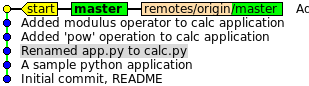
\includegraphics[width=\linewidth]{gitk-start.png}
  \label{fig:gitk-start}
  \caption{Notre projet affiché dans Gitk. Il n'y a qu'un branche locale avec un historique linéaire.}
\end{marginfigure}

\begin{lstlisting}[style=BashInputStyle]
  $ gitk --all
\end{lstlisting}

Cette alternative est un moyen très simple et rapide pour obtenir un aperçu de toutes les branches: locales et remotes (et de plusieurs remotes si présents).
Dans Gitk, les branches locales sont vertes, la branche local courant est en gras sur fond vert, et les branches remote sont préfixées de texte sur fond rose.
Notre projet dispose aussi d'un label jaune, qui est un \texttt{tag}.
\marginnote{Vous ne pouvons pas d\'eplacer un tag, mais il est toujours possible de le supprimer et de le red\'efinir ailleurs. Attention que cela entra\^inera des complications si le tag est d\'ejà partag\'e sur d'autres clients Git (ils ne pourront pas d\'etecter ce d\'eplacement de tag sans le supprimer localement).}
Comme une branche, un \texttt{tag} n'est autre qu'une étiquette sur un commit, la différence principale étant qu'un tag est supposé être permanent pour identifier un point important dans l'historique du projet (publication d'un nouvelle version de code, étape de développement...), tandis qu'une branche évolue de commit en commit.

\subsection{L'état du working tree}

Nous allons bientôt appliquer des changements au projet.
Une commande utile pour suivre l'état des differents fichiers dans Git est \texttt{git status}:

\begin{lstlisting}[style=BashInputStyle]
  $ git status
\end{lstlisting}

Comme nous n'avons encore rien modifié, la sortie de \texttt{git status} est triviale:

\begin{lstlisting}[style=BashInputStyle]
  On branch master
  nothing to commit (working directory clean)
\end{lstlisting}

Git status est plus bavard losqu'on commence à faire des modifications.
La sortie de \texttt{git status} groupera les fichiers par catégories selon leur état: \textbf{stages}, \textbf{modified} et \textbf{untracked}.

\section{Appliquons nos premières modifications sur master}

Dans beaucoup de workflows, il n'est pas recommandé de travailler directement sur la branche \texttt{master}.
Nous allons ignorer cette règle de bonne pratique pour le moment pour simplifier.
Plus tard, nous appliquerons toujours des modifications sur des branches isolées et répatrieront les modifications dans \texttt{master} quand désirable.

\subsection{Git add pour indexer un fichier non-suivi}

Créons un nouveau fichier avant d'exécuter \texttt{git status}:

\begin{lstlisting}[style=BashInputStyle]
  $ echo hello > newfile.txt
  $ git status
  # On branch master
  # Untracked files:
  #   (use "git add <file>..." to include in what will be committed)
  #
    §newfile.txt§
  nothing added to commit but untracked files present (use "git add" to track)
\end{lstlisting}

Git status est plus verbeux, il renseigne qu'il y a un nouveau fichier dans le working tree, non-versionné.
Tous les fichiers ajoutés au working tree sont \texttt{untracked}, et le resteront tant qu'on ne les ajoute pas explicitement au repository Git.

\begin{marginfigure}%
  \centering
  
\includegraphics[width=\linewidth]{gitadd-schema.pdf}
  \label{fig:gitadd}
  \caption{Git add sur un fichier indexera toutes les modifications faites dans ce fichier. Cela ajoutera également un fichier non-versioné à l'index.}
\end{marginfigure}

\begin{lstlisting}[style=BashInputStyle]
  $ git add newfile.txt
  $ git status
    On branch master
    Changes to be committed:
      (use "git reset HEAD <file>..." to unstage)
  
    `new file:   newfile.txt`
\end{lstlisting}

\subsection{Notre premier commit}

L'index (aussi appelé \texttt{staging area}) est propre à Git et le rend très puissant.
\marginnote{La notion de commit existe aussi en SVN mais est très différente. Un commit SVN est non-réversible et applique des changements sur le repository remote. Un commit Git est une opération local qui peut être aisément modifiée ultérieurement, avant d'être partagée sur un serveur distant.}
Des modifications successives peuvent être appliquées jusqu'à ce que le développeur soit satisfait du contenu, et est prêt à effectuer un \texttt{commit}.
Committer des changes créera un nouveau point dans l'historique du projet, et déplacera le pointeur HEAD et la branche courante sur ce nouveau commit.

\begin{marginfigure}%
  \centering
  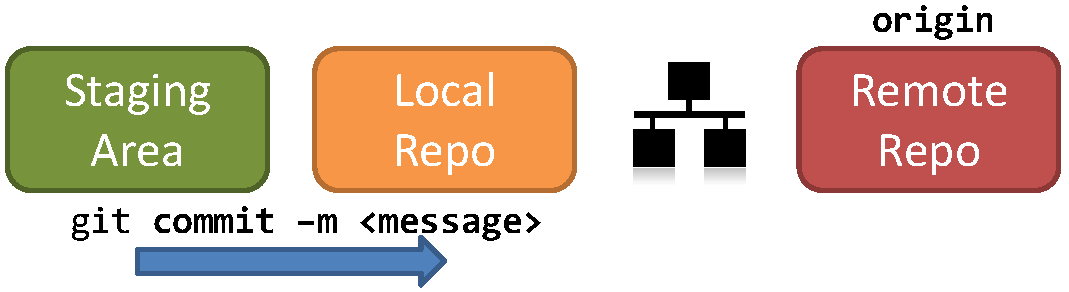
\includegraphics[width=\linewidth]{gitcommit-schema.pdf}
  \label{fig:gitcommit}
  \caption{Git commit crée un nouveau point dans l'historique, en appliquant les changements contenus dans l'index.}
\end{marginfigure}

\begin{lstlisting}[style=BashInputStyle]
  $ git commit -m "Added new file"
  [master 494822d] Added new file
   1 file changed, 1 insertion(+)
   create mode 100644 newfile.txt
\end{lstlisting}

Ci-dessous, le message de commit est appliqué directement dans la commande avec l'option \texttt{-m}, mais peut également être encodé dans un éditeur texte en omettant l'option.

\subsection{Git add pour indexer des modifications dans des fichiers suivis}

Ajoutons plus de contenu à notre nouveau fichier:

\begin{lstlisting}[style=BashInputStyle]
  $ echo "hello again" >> newfile.txt
  $ git status
    On branch master
    Your branch is ahead of 'origin/master' by 1 commit.
  
    Changes not staged for commit:
      (use "git add <file>..." to update what will be committed)
      (use "git checkout -- <file>..." to discard changes in working directory)
   
    §modified:   newfile.txt§
   
no changes added to commit (use "git add" and/or "git commit -a")
\end{lstlisting}

Tapper \texttt{git commit} à ce stade ne créera aucun commit car les modifications apportées au fichier n'ont pas été indexées.
Il est possible d'indexer toutes les modifications présentes dans le ficheir avec la même commande \texttt{git add}, précédemment utilisées pour indexer un fichier non-versionné:

\begin{lstlisting}[style=BashInputStyle]
  $ git add newfile.txt
  $ git status
    On branch master
    Your branch is ahead of 'origin/master' by 1 commit.
  
    Changes to be committed:
      (use "git reset HEAD <file>..." to unstage)
  
    `modified:   newfile.txt`
 
\end{lstlisting}

A présent, un \texttt{git commit} appliquera les modifications indexées dans un nouveau commit:

\begin{marginfigure}%
  \centering
  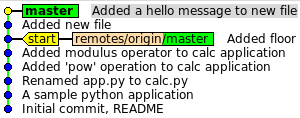
\includegraphics[width=\linewidth]{gitk-2commits.png}
  \label{fig:gitk2commits}
  \caption{Gitk after 2 commits on the local master branch}
\end{marginfigure}

\begin{lstlisting}[style=BashInputStyle]
  $ git commit -m "Added a hello message to new file"
  [master 25d79d3] Added a hello message to new file
   1 file changed, 1 insertion(+)
\end{lstlisting}

\subsection{Git add -p: l'indexation granulaire}

L'une des techniques les plus propres pour indexer des modifications en ligne de commande et l'option \texttt{-p} de \texttt{git add}:

\begin{lstlisting}[style=BashInputStyle]
  $ git add -p
\end{lstlisting}

Cela ne prend pas de nom de fichier en argument.
\texttt{git add -p} initiera une session interactive durant laquelle chaque modification non-indexée (\texttt{hunk}) sera affichée. Pour chaque \texttt{hunk}, l'utilisateur décidera de l'ajouter à l'index ou de le laisser en état \texttt{modified}. \marginnote{Choix sur hunks de \texttt{git add -p}: \textbf{y}: indexer, \textbf{n}: ne pas indexer, \textbf{d}: ne pas indexer et sauter le reste du fichier, \textbf{s}: découper en \texttt{hunks} plus petits, si possible, et redemander.}
Cette commande est très pratique car elle permet d'indexer des lignes de code plutôt que des fichiers entiers, ce qui veut dire que vous pouvez indexer un fichier partiellement.
De cette façon, il est possible d'isoler des features dans des commits séparés, même si ces modifications partagent les mêmes fichiers.
La sessions interactive s'achèvera lorsque toutes les modifications seront passées en revue.

Supposons que nous avons deux modifications dans \texttt{calc.py} et que nous avons sélectionné \textbf{y} pour seulement l'une d'entre elles dans un \texttt{git add -p}.
Le fichiers contiendra à la fois des lignes modified et des lignes indexées:

\begin{lstlisting}[style=BashInputStyle]
  $ git status
    On branch master
    Your branch is ahead of 'origin/master' by 2 commits.
  
    Changes to be committed:
      (use "git reset HEAD <file>..." to unstage)
  
    `modified:   python/calc.py`
  
    Changes not staged for commit:
      (use "git add <file>..." to update what will be committed)
      (use "git checkout -- <file>..." to discard changes in worki...
  
    §modified:   python/calc.py§
\end{lstlisting}

Un \texttt{git commit} ici appliquera l'index dans un nouveau commit, et laisser la partie \texttt{modified} du fichier indemne.
Nous avons déjà exploré les commits, donc restons dans cet état pour explorer la commande \textbf{diff}.

\marginnote{\texttt{git diff} affiche la différence entre le contenu modifié et HEAD. Les changements déjà indexés ne sont pas pris en compte.}
\begin{lstlisting}[style=BashInputStyle]
  $ git diff
  diff --git a/python/calc.py b/python/calc.py
  index b66135e..9178e52 100644
  --- a/python/calc.py
  +++ b/python/calc.py
  @@ -17,6 +17,7 @@ def mul(op1, op2):
   def div(op1, op2):
     return op1 / op2
 
  `+ New comment, I will not stage it for now`
   def pow(op1, op2):
     return op1 ** op2
 \end{lstlisting}
\marginnote{\texttt{git diff} avec l'option \textbf{cached} fait l'inverse: cela affiche la différence entre le contenu déjà indexé et HEAD et ignore le contenu non-indexé.}
 \begin{lstlisting}[style=BashInputStyle]
  $ git diff --cached
  diff --git a/python/calc.py b/python/calc.py
  index c27b82f..b66135e 100644
  --- a/python/calc.py
  +++ b/python/calc.py
  @@ -2,6 +2,7 @@ import os
   import sys
   import argparse
 
  `+ New comment. I will stage this first`
   choices_cmd = ['add', 'sub', 'mul', 'div', 'pow', 'mod', 'floor']
 
   def add(op1, op2):
\end{lstlisting}

\subsection{Indexer tous les modified et untracked en une commande}

Même si je déconseille souvent son usage, il est possible d'indexer tous les fichiers untracked et modifiés en une seule commande:

\begin{lstlisting}[style=BashInputStyle]
  $ git add -A
\end{lstlisting}

\subsection{Committer toutes les modifications en une fois}

Un autre racourcis bon à connaître mais dont il ne faut pas abuser est la possibilité d'indexer et committer toutes les modifications non-indexées. Ceci est moins extrême que \texttt{git add -A} car les fichiers untracked ne seront pas indexés.

\begin{marginfigure}%
  \centering
  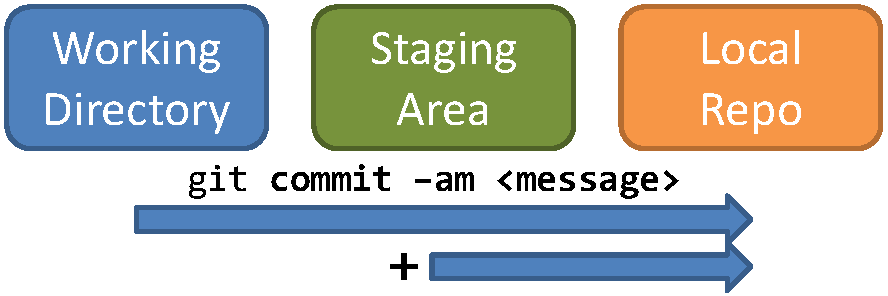
\includegraphics[width=\linewidth]{gitcommit-am-schema.pdf}
  \label{fig:gitcommit-am}
  \caption{Git commit -am indexe toutes les modifications et applique un commit automatiquement.}
\end{marginfigure}
\begin{lstlisting}[style=BashInputStyle]
  $ git commit -am "One big commit"
\end{lstlisting}

Je préfère éviter ces deux dernières commandes car les commits devraient contenir des changements isolés et il est rare de travailler exclusivement sur un feature en particulier sans introduire de mo-difications superflues.
L'option \texttt{-a} de \texttt{git commit} ne permet pas de passer en revue l'état de l'index avant d'appliquer les changement.
Le fait de découpler les phases d'index et de commit permettent de visualiser l'index à l'aide de commandes telles que:

\begin{lstlisting}[style=BashInputStyle]
  $ git diff --cached
\end{lstlisting}

\subsection{Désindexer des changements}

Pour désindexer quelque chose, \texttt{git reset} est en général le plus pratique. \marginnote{\texttt{git reset} sans arguments va en effet désindexer tout l'index et restaurer le contenu de l'index dans son état d'origine (modified, untracked ou non-supprimé si en désindexer une opération de suppression de fichier).}
La commande \texttt{reset} a des comportement très différents selons les options; ici, nous utilisons le reset normal (ni \texttt{hard}, ni \texttt{soft}) pour désindexer nos modifications sans les supprimer.

%TODO: review this note, seems fishy
%\marginnote{Although it's technically possible to combine \texttt{[tree-ish]} and \texttt{[file]} options to git reset, this will not actually delete the commit if there are other non-reset changes in the commits. Thus the content is reset as desired, but applied this reset requires to stage and commit the modifications in new commits. Git revert has a similar behavior in the sense that we are adding commits to actually undo work.}

\begin{lstlisting}[style=BashInputStyle]
  $ git reset 
\end{lstlisting}

L'explications sur \texttt{git reset} n'est pas complète.
Comme beaucoup de commandes git, le reset prend un \textbf{tree-ish} comme argument optionnel, et suppose \texttt{HEAD} lorsque ce dernier est omis.
Le \texttt{git reset} général défera les commits depuis l'état actuel juqu'au commit référencé par le tree-ish (sans défaire ce dernier).

\begin{lstlisting}[style=BashInputStyle]
  $ git reset [tree-ish]
\end{lstlisting}

Enfin, il est possible de désindexer un fichier en particulier:

\begin{lstlisting}[style=BashInputStyle]
  $ git reset [file]
\end{lstlisting}

\section{Dé-versionner et supprimer des fichiers}

Une suppression de fichier est une modification comme une autre dans Git.
Il y a deux façon de supprimer un fichier.
La méthode \textit{propre et recommandée} est de supprimer un fichier ou dossier directement avec la commande Git.
Il est aussi possible de supprimer des fichiers ou dossiers sur son système de fichiers sans passer par Git.
Même s'il est assez facile d'en avertir Git par la suite, ce n'est pas la méthode préconisée.
\marginnote{Utilisateurs SVN: oui, cela peut sembler magique}
Nous allons aborder les deux méthodes dans la prochaine section.

\subsection{Supprimer des fichiers via Git}

La moyen le plus propre pour supprimer un fichier du disque et de repository Git est d'utiliser \texttt{git rm}:

\begin{lstlisting}[style=BashInputStyle]
  $ git rm <file>
\end{lstlisting}

Cela fait deux choses: le fichier sera supprimé du disque, et la suppression est \textbf{indexées} dans Git.
Le prochain commit contiendra donc, parmi ses modifications, le fait que le fichier en question est supprimé.

Si vous souhaitez retirer un fichier de Git sans le supprimer localement, il faut rajouter l'option \texttt{cached}:

\begin{lstlisting}[style=BashInputStyle]
  $ git rm --cached <file>
\end{lstlisting}

\marginnote{rm cached est pratique pour déversionner des fichiers que vous auriez oublié d'inclure dans votre .gitignore}
Git indexera le fait que le fichier doit être supprimé au prochain commit, mais ne touchera pas à la copie locale du fichier.

\subsection{Supprimer des fichiers en dehors de Git}

Donc, que se passe-t-il si on supprimer des fichiers sans en avertir Git?
Git détectera le contenu supprimé, et vous le dira dans votre prochain \texttt{git status}

\begin{lstlisting}[style=BashInputStyle]
  $ rm README.md
  $ git status
  On branch master
  Your branch is up-to-date with 'origin/master'.

  Changes not staged for commit:
    (use "git add/rm <file>..." to update what will be committed)
    (use "git checkout -- <file>..." to discard changes in working directory)

      §deleted:    README.md§

  no changes added to commit (use "git add" and/or "git commit -a")
\end{lstlisting}

\marginnote{contrairement à \texttt{git rm README.md}, qui indexera la suppression.}
La contenu supprimé sera considéré comme une modification: son état sera donc \texttt{modified} plutôt que \texttt{staged}.
Il est possible d'exécuter \textit{git rm} sur chaque fichier supprimé, même s'il n'est déjà plus présent sur le disque, pour demander à Git d'indexer cette suppression.

Cette opération peut s'avérer fastidieuse s'il y a beaucoup de suppressions.
Il y a des raccourcis, en commençant par \texttt{git add -u <pathspec>}, qui indexe des modifications et suppressions parmi les fichiers précisés dans l'option <pathspec>. 
\marginnote{c'est le moment idéal de parcourir la documentation de git add, avec \texttt{git add --help}}
Si celle-ci n'est pas présente, la commande couvre les fichiers versionnés de tout le working tree. Sans arguments supplémentaires, \texttt{git add -A} a un comportement similaire.

\begin{lstlisting}[style=BashInputStyle]
  $ git add -u
  $ git add -A # equivalent without pathspec
\end{lstlisting}

Dans le cas de fichiers supprimés, \texttt{git add -u} indexera chaque suppression. Le prochain commit appliquera toutes les suppressions.

\section{Pusher des contributions sur un remote}

Jusqu'ici, nous avons fait évoluer le projet sur une branche \texttt{master} locale.
Toutes ces modifications sont locales à notre machine et n'ont pas été partagées.

\begin{marginfigure}%
  \centering
  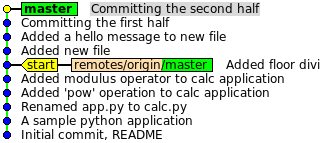
\includegraphics[width=\linewidth]{gitcommit-pre-push.png}
  \label{fig:gitcommit-pre-push}
  \caption{Etat des repos local et remote avant le push. La branche master locale est 4 commits en avance sur celle d'origin}.
\end{marginfigure}
\begin{marginfigure}%
  \centering
  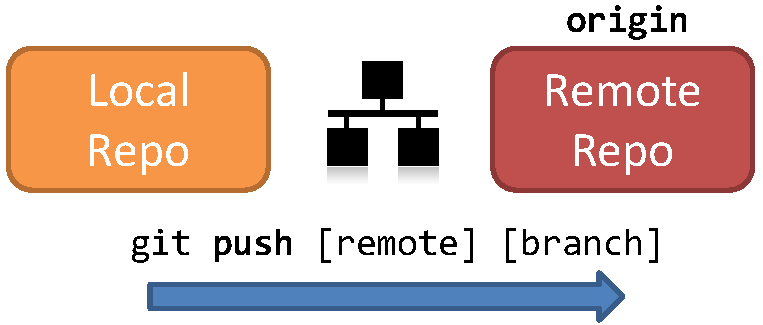
\includegraphics[width=\linewidth]{gitpush-schema.pdf}
  \label{fig:gitpush-schema}
\end{marginfigure}
\begin{marginfigure}%
  \centering
  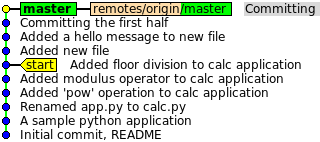
\includegraphics[width=\linewidth]{gitcommit-post-push.png}
  \label{fig:gitcommit-post-push}
  \caption{Après le push vers origin, les deux branches master sont au même stade.}
\end{marginfigure}

La commande \texttt{git push} sert à envoyer des branches individuelle depuis le repository local vers un repository distant.
La commande renvoie typiquement:

\begin{lstlisting}[style=BashInputStyle]
  $ git push origin master 
  Counting objects: 17, done.
  Delta compression using up to 8 threads.
  Compressing objects: 100% (10/10), done.
  Writing objects: 100% (14/14), 1.29 KiB, done.
  Total 14 (delta 4), reused 0 (delta 0)
  To git@gitlab.server.com:login/lesson1
     71aaf45..37b9258  master -> master
\end{lstlisting}

Git push n'est permis que si la branche remote sur laquelle on pousse n'a pas été modifiée entre temps.
Autrement dit, l'opération réussira \textit{uniquement si la pointe de la branche remote est un ancêtre directe de la branche locale qu'on pousse}.

Les cas où la branche remote a été mise à jour (par quelqu'un d'autre, en général) et qu'il pas possible de push, sont adressés dans les workflows multi-utilisateurs qui seront abordés plus tard.
\marginnote{J'utilise le terme intégrer pour rester général. Il y a plusieurs façons de le faire, comme merge, rebase, hard reset reset...}
En 2 mots, les modifications doivent d'abord être rapatriées localement puis intégrée avec notre travail avant de pouvoir contribuer.

\section{Passer par une branche feature}

Jusqu'à présent, nous avons travaillé sur master.
Nous allons conclure cette session en montrant comment travailler sur une branche séparée et de fusionner ces denières dans \texttt{master} une fois qu'elles sont stables.

\subsection{Les branches: très agiles}

Créer une branche dans Git est très rapide: cela revient à ajouter une étiquette sur un commit existant.
\marginnote{C'est fondamentalement différent de certains autres SCMs, où la création d'une branche peut être une processus très longue de copie entière de working tree dans un nouveau dossier.}
Le working tree demeure inchangé lorsqu'on crée une branche.
\begin{marginfigure}%
  \centering
  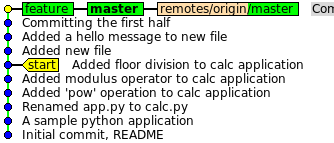
\includegraphics[width=\linewidth]{gitbranch-feature.png}
  \label{fig:gitbranch-feature}
  \caption{Nouvelle branche = nouvelle étiquette}
\end{marginfigure}
\begin{lstlisting}[style=BashInputStyle]
  $ git branch -a
  * `master`
    §remotes/origin/HEAD -> origin/master§
    §remotes/origin/master§

    $ git branch feature

  $ git branch -a
    feature
  * `master`
    §remotes/origin/HEAD -> origin/master§
    §remotes/origin/master§
\end{lstlisting}

Nous avons une nouvelle branche locale appelée \texttt{feature} et qui pointe sur le même commit que la branche \texttt{master}.
\marginnote{Ne soyez pas déstabilisé par le fait qu'il n'y a pas "branchement" dans l'historique après la création d'une branche. En réalité, nous n'avons encore rien modifié: les deux branches sont strictement identiques.}
Nous ne sommes pas encore prêt à appliquer des changements, car \texttt{git branch} et \texttt{git status} nous renseignent que nous sommes encore sur la branche \texttt{master}
Afin de faire progresser la branche \texttt{feature} plutôt que \texttt{master} aux prochains commits, il faut utiliser \texttt{git checkout}:

\begin{lstlisting}[style=BashInputStyle]
  $ git checkout feature
  $ git branch -a
  * feature
    master
    remotes/origin/HEAD -> origin/master
    remotes/origin/master
\end{lstlisting}

\subsection{Intégrer une branche dans master}

Nous pouvons maintenant ajouter des commits sur notre branche \texttt{feature}, comme nous l'avons fait auparavant pour \texttt{master}.
Lorque nous sommes satisfait de notre travail, il est temps d'intégrer la branche \texttt{feature} dans \texttt{master}.
Nous n'allons pas trop nous attarder sur ces opérations pour le moment, mais voici déjà une possibilité pour réaliser l'intégration:

\begin{marginfigure}%
  \centering
  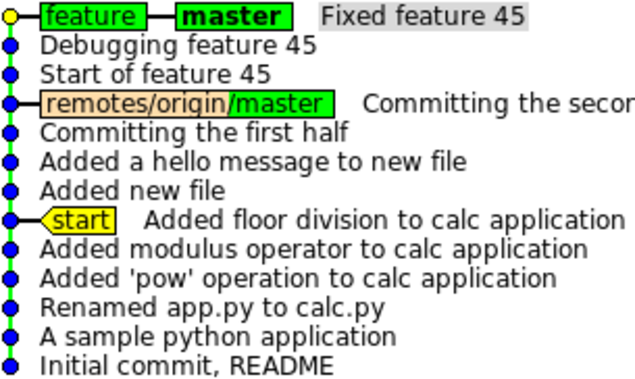
\includegraphics[width=\linewidth]{gitmerge-ff.pdf}
  \label{fig:gitmerge-ff}
  \caption{Merge, en mode fast-forward}
\end{marginfigure}

\begin{lstlisting}[style=BashInputStyle]
  $ git checkout master
  $ git merge feature
\end{lstlisting}

Si \texttt{master} n'a pas évolué depuis que nous avons créé la branche, elle se trouvera en ancêtre direct de notre branche, \texttt{feature}, et pourra être \textbf{fast-forwarded} vers \texttt{feature}.
S'il est préférable d'avoir un branchement explicite dans l'historique, il est possible de forcer la création d'un commit dit \texttt{merge commit} avec \texttt{no-ff}:

\begin{marginfigure}%
  \centering
  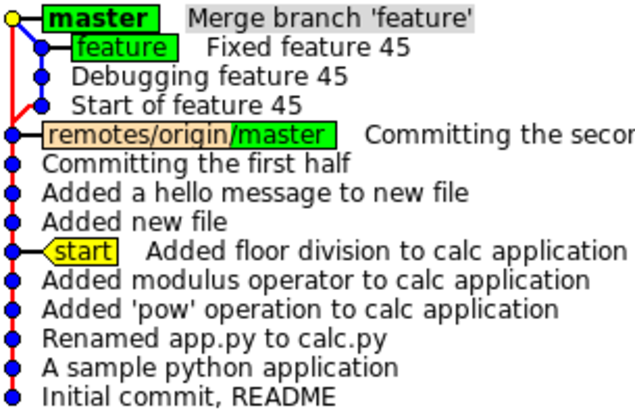
\includegraphics[width=\linewidth]{gitmerge-noff.pdf}
  \label{fig:gitmerge-noff}
  \caption{Merge avec no-fast-forward force la créaton d'un merge commit}
\end{marginfigure}

\begin{lstlisting}[style=BashInputStyle]
  $ git checkout master
  $ git merge feature --no-ff
\end{lstlisting}

Ce commit additionel a 2 parents: le dernier commit de chaque branche avant la fusion.
En revanche, si master avait évolué depuis le branchement de feature, l'opération de merge aurait automatiquement créé ce merge commit.

Dans la prochaine session, nous allons explorer les workflows avec branches multiples, développeurs multiples et aborder d'autres façons d'intégrer des changements, tels que \textbf{rebase}.

\bibliography{../common/refs}
\bibliographystyle{plainnat}

\end{document}


% \marginnote{}